\documentclass[a4paper]{article}
\usepackage[utf8]{vietnam}
\usepackage{graphicx}
\usepackage{amssymb}
\usepackage{amsmath}
\usepackage{scrextend}
\usepackage{tcolorbox}
\usepackage{setspace}
\usepackage{times}
\usepackage{listings}
\usepackage{tvietlistings}
\usepackage{xcolor}
\usepackage{indentfirst}
\setlength{\parindent}{0.5cm}

%New colors defined below
\definecolor{codegreen}{rgb}{0,0.6,0}
\definecolor{codegray}{rgb}{0.5,0.5,0.5}
\definecolor{codepurple}{rgb}{0.58,0,0.82}
\definecolor{backcolour}{rgb}{0.95,0.95,0.92}

%Code listing style named "mystyle"
\lstdefinestyle{mystyle}{
	backgroundcolor=\color{backcolour},   commentstyle=\color{codegreen},
	keywordstyle=\color{magenta},
	numberstyle=\tiny\color{codegray},
	stringstyle=\color{codepurple},
	basicstyle=\ttfamily\footnotesize,
	breakatwhitespace=false,         
	breaklines=true,                 
	captionpos=b,                    
	keepspaces=true,                 
	numbers=left,                    
	numbersep=5pt,                  
	showspaces=false,                
	showstringspaces=false,
	showtabs=false,                  
	tabsize=2
}

%"mystyle" code listing set
\lstset{style=mystyle}

\onehalfspacing
\textwidth=16 cm
\oddsidemargin=0 cm
\evensidemargin=1 cm
\topmargin= -1 cm

\renewcommand\thesection{Câu \alph{section}.}
\renewcommand\thesubsection{\roman{subsection}.}

\title{BIỄU DIỄN TRI THỨC\\ Bài tập 2}
\author{Nhóm 07}
\date{May 29th, 2021}

\begin{document}
	\maketitle
	\begin{center}
		\LARGE{\textbf{Bài 2\\Bài toán điều chế các chất hóa học}}
	\end{center}
	
	\section{Tổ chức lưu trữ cho miền tri thức} 	
	
	Với phạm vi bài toán, miền tri thức thu thập sẽ nằm trong giới hạn đủ để giải quyết yêu cầu bài toán bao gồm một số những phương trinh hóa học cần thiết để điều chế \texttt{Na$_2$SO$_4$}, \texttt{H$_2$SO$_4$}, \texttt{HCl} và \texttt{Na} từ \texttt{S}, \texttt{H$_2$O},và \texttt{NaCl} như:
	
	\texttt{NaCl} = \texttt{Na} + \texttt{Cl$_2$}  
	
	\texttt{Na} + \texttt{H$_2$SO$_4$} = \texttt{Na$_2$SO$_4$} + \texttt{SO$_2$} + \texttt{H$_2$O}
	
	Miền tri thức các phương trình phản ứng hóa học trên được lưu trữ trong tập tin dưới định dạng text (\textbf{\textit{.txt}}) được minh họa trong hình \ref{fig-2a:mien-tri-thuc}. 
	\begin{figure}[h]
		\centering
		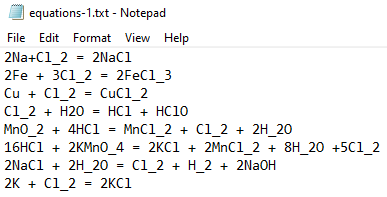
\includegraphics[width=0.7\linewidth]{images/2a_mien-tri-thuc}
		\caption{Minh họa miền tri thức trong tập tin định dạng text}
		\label{fig-2a:mien-tri-thuc}
	\end{figure}
	
	Nhóm em sử dụng kiến thức về Lập trình hướng đối tượng để tổ chức lưu trữ và xử lý tự động các tri thức trên máy tính. Lớp đối tượng cơ bản \texttt{EQUATION} biểu diễn phương trình hóa học được định nghĩa như sau:
	\begin{lstlisting}[language=Python, caption=Lớp đối tượng \texttt{EQUATION}]
		class EQUATION:
			vars_VP = []
			vars_VT = []
			
			#Khai báo lớp đối tượng
			def __init__(self, name, vars_VT, vars_VP):
				self.name = name
				self.vars_VT = vars_VT
				self.vars_VP = vars_VP
			
			# Tổng số chất đã biết bên vế trái của phương trình hóa học
			def get_num_vars(self):
				return len(self.vars_VT)
	\end{lstlisting}
	Trong đó, các biến có nghĩa:
	\begin{itemize}
		\item \texttt{name} có dạng "công thức \texttt{i}" với \texttt{i} là số thứ tự của công thức đó trong miền tri thức tính từ 1.
		\item \texttt{vars\_VT} là bao gồm các chất bên trái dấu bằng (=) của từng tri thức, gọi là các \textbf{chất đã biết}.
		\item \texttt{vars\_VP} là bao gồm các chất bên phải dấu bằng (=) của từng tri thức, gọi là các \textbf{chất cần điều chế}.
	\end{itemize}
	
	\section{Trình bày thuật giải}
	\begin{lstlisting}[language=Python, caption=Thuật giải mạng ngữ nghĩa điều chế]
		def solve(self):
			#Đặt cờ truy vết "giải được bài toán"
			flag = True
			while flag:
				flag = False
					
				#Duyệt từng phương trình
				for equation in self.equations:
					#Lấy chất điều chế bên VT phương trình
					known_var = self.get_known_vars(equation)
					
					#Nếu như 1 node (chất) có thể điều chế được (khác -1)
					if known_var != -1:
						#Kích hoạt node có thể điều chế được
						self.active_var(known_var)
						
						#Tiến thành lưu lại pt có thể điều chế
						self.add_step(known_var, equation)
						flag = True
						
						# Kiểm tra xem đã giải bài toán thành công chưa?
						if self.is_success():
							temp = []
							solutions = temp
							# Trả về lời giải đến đích
							for step in self.steps:
								solutions.append(step)
							return [True, solutions]
						
				# Nếu không giải được trả về yêu cầu thêm thông tin, tri thức
				return [False, "Bài toán không thể giải, hãy bổ sung thêm thông tin hoặc tri thức."]
	\end{lstlisting}
	
	\section{Cài đặt chương trình}
	\subsection{Thông tin chương trình}
		\begin{enumerate}
			\item Tên chương trình: \textbf{Chemistry Lab - Nhóm 07}
			\item Chương trình thực thi: \texttt{chemistry-lab\_Nhom07.exe}
			\item Video demo: \texttt{chemistry-lab\_Nhom07-Demo.mp4}
			\item Ngôn ngữ lập trình: $Python$
			\item Thiết kế giao diện người dùng: $PyQt5$
			\item Các tính năng chính:
			\begin{itemize}
				\item Trình bày từng bước điều chế các chất hóa học cần thiết.
				\item Có thể xử lý trên miền tri thức linh hoạt với các phương trình hóa học có hoặc không có hệ số cân bằng.
			\end{itemize}
		\end{enumerate}
	
	\subsection{Hướng dẫn sử dụng}
		\begin{figure}[h]
			\centering
			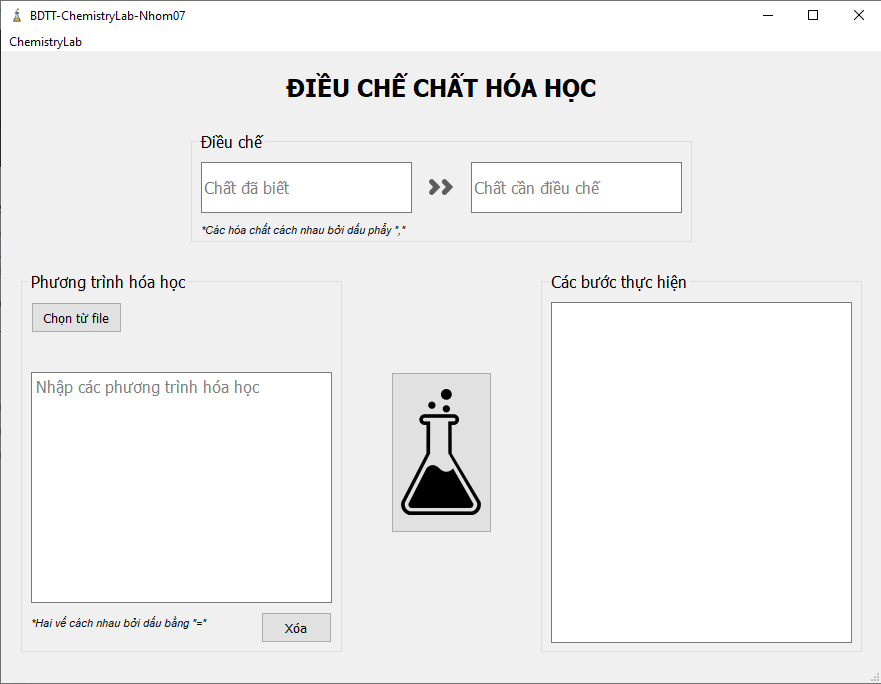
\includegraphics[width=0.7\linewidth]{images/app-ui}
			\caption{Màn hình giao diện Chemistry Lab - Nhóm 07}
			\label{fig:app-ui}
		\end{figure}
		\begin{itemize}
			\item \textbf{Quy ước định dạng phương trình hóa học và hóa chất:} 
			\begin{itemize}
				\item Các chất hóa học như \texttt{Cl$_2$, H$_2$O, SO$_2$,...} sẽ được đưa vào dưới dạng \texttt{Cl\_2, H\_2O, SO\_2,...}
				\item Dấu mũi tên trong các phương trình hóa học sẽ được thay bởi dấu bằng "=". Ví dụ: \texttt{2Na+Cl$_2$ $\rightarrow$ 2NaCl} sẽ được đưa vào dưới dạng \texttt{2Na+Cl\_2 = 2NaCl}
			\end{itemize}
		
			\item \textbf{Điều chế:} Người dùng nhập các chất hóa học đã có (nguyên liệu điều chế) vào ô \textcolor{blue}{\texttt{Chất đã biết}} (bên trái), và nhập các chất hóa học cần điều chế vào ô \textcolor{blue}{\texttt{Chất cần điều chế}} (bên phải). 
			
			Trong quá trình nhập liệu, người dùng sử dụng \textbf{dấu phẩy (,)} để ngăn cách các hóa chất.
			
			\underline{Ghi chú}: chương trình đã mặc định có chất \texttt{O$_2$} ở \textcolor{blue}{\texttt{Chất đã biết}}, vì chất này có sẵn trong không khí.
			
			\item \textbf{Phương trình hóa học:} Người dùng có thể đưa tri thức (các phương trình hóa học) vào chương trình bằng 2 cách:
			\begin{itemize}
				\item Nhập trực tiếp: người dùng nhập các phương trình hóa học, theo đúng định dạng quy ước, vào ô trống. Các phương trình ngăn cách nhau bởi kí hiệu ngắt dòng (\texttt{<Enter>}).
				
				\item Nhập từ file: người dùng chọn \textcolor{blue}{\texttt{Chọn từ file}} và chọn tệp tin chứa các phương trình hóa học cần đưa vào, lúc này các phương trình hóa học trong tệp tin sẽ được hiển thị ở ô trống phía dưới.
				
				\underline{Lưu ý}: chỉ có thể chọn \textbf{một} tệp tin (định dạng text \textbf{\textit{.txt}}) và không thể chỉnh sửa trong ô trống.
			\end{itemize}
		
			Người dùng có thể chọn \textcolor{blue}{\texttt{Xóa}} để xóa tất cả các phương trình hóa học vừa nhập.
			
			\item Sau khi cung cấp đủ thông tin ở hai phần \textbf{Điều chế} và \textbf{Phương trình hóa học}, người dùng chọn nút có hình "lọ hóa chất" để chương trình tiến hành điều chế, kết quả sẽ được hiển thị ở phần \textbf{Các bước thực hiện}.
		\end{itemize}
	
	\subsection{Một số hình ảnh}
		\begin{figure}[h]
			\centering
			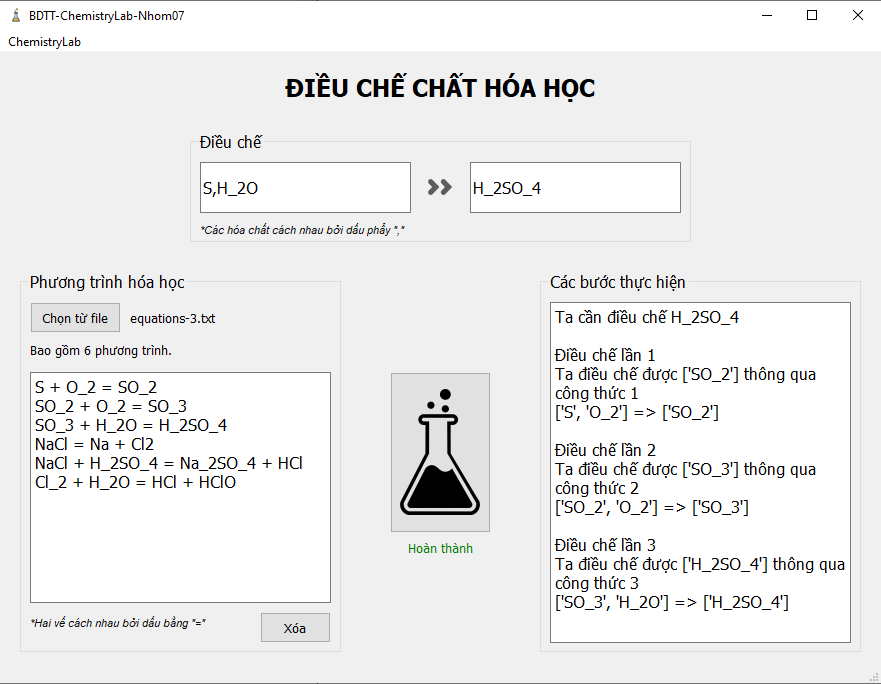
\includegraphics[width=0.7\linewidth]{images/app-done-2}
			\caption{Các bước thực hiện để điều chế \texttt{H$_2$SO$_4$} từ \texttt{S} và \texttt{H$_2$O}}
			\label{fig:app-done-2}
		\end{figure}
		
		\begin{figure}
			\centering
			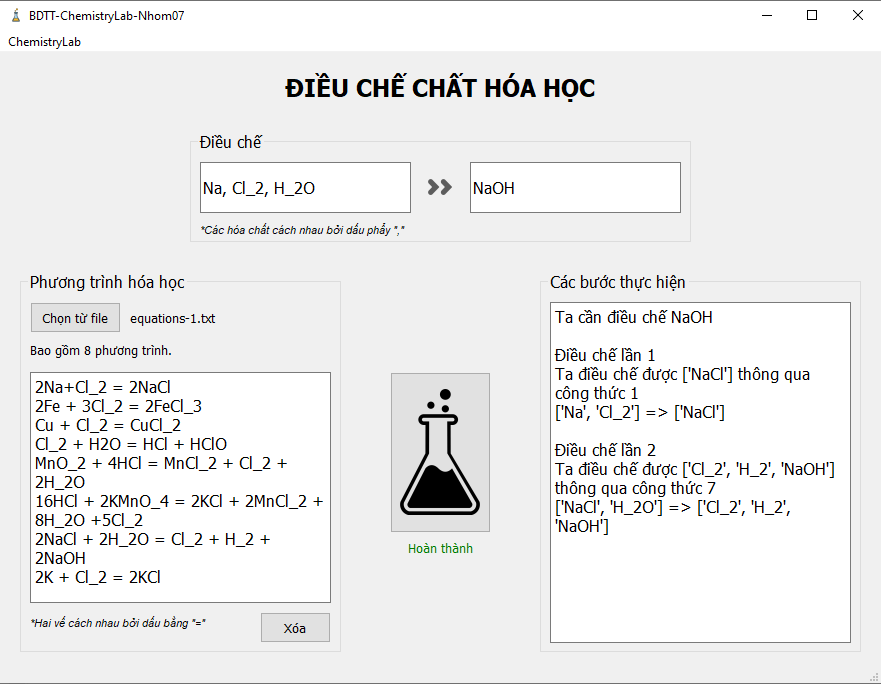
\includegraphics[width=0.7\linewidth]{images/app-done}
			\caption{Minh họa điều chế $NaOH$ với các chất đã cho $Na$, $Cl_2$, $H_2O$}
			\label{fig:app-done}
		\end{figure}
		
		\begin{figure}[h]
			\centering
			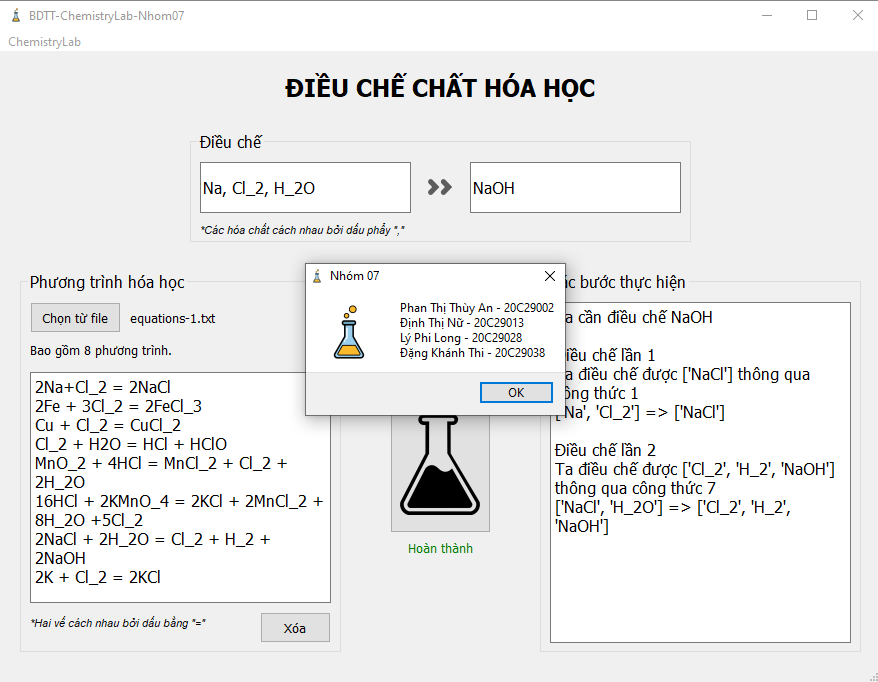
\includegraphics[width=0.7\linewidth]{images/app-authors}
			\caption{Nhóm học viên thực hiện}
			\label{fig:app-authors}
		\end{figure}


\end{document}